%!TEX root = ../fbi.tex

\section{Conclusion and Discussion}

\appendix

\section{Determining the edge action of the symmetry using MPS}
\label{Appendix:MPS}

We can use the formalism of MPS to assign an action
of the symmetry on the Schmidt states, and in particular for the charge and 
translation on-site symmetries the Schmidt states can be simultaneously assigned
charge and translation quantum numbers. This method of discovering the symmetry 
action will reproduce the action discussed in \ref{sec:ES} and quantum numbers used
in the spectra plots shown in Fig.~\ref{fig:ESL910}.
  
Let's discuss this formalism briefly. In addition,
we will discuss a generalization of this method that allows us to numerically
determine the symmetry action of inversion symmetry on the Schmidt states,
as in Section~\ref{sec:symmetry}. 
Both of these discussions follow Ref.~\onlinecite{pollmann2010}.

These discussions start by finding tensors $\Gamma, \Lambda$ representing the 
so-called canonical form of the MPS, as
originally detailed in \cite{perezgarcia2008}. This canonical form provides the Schmidt
decomposition at each site in the lattice.
\beq
\ket{\psi} = \sum\limits_{\{p_i\}} \ldots \Lambda \Gamma_{p_0} \Lambda \Gamma_{p_1} \Lambda \Gamma_{p_2} \Lambda \ldots \ket{... p_0 p_1 p_2 ...}.
\eeq
As a reminder, each physical leg represents all $2W$ physical sites on a cylinder slice,
and each virtual leg represents all virtual indices that connect cylinder slices.
The change of basis to canonical form generally mixes the Hilbert spaces from these
virtual legs, so the resulting basis won't be local around the circumference
of the cylinder.

Each on-site symmetry of the wavefunction $U_g = \otimes_i u^i_g$, with $U_g
\ket{\psi} = e^{i \Theta_g} \ket{\psi}$ is assigned an operator $V_g$ that
acts on the virtual leg of the MPS, that satisfies the equation
\begin{center}
\beq
\label{eq:onsitesym}
\eeq
\vskip-5em
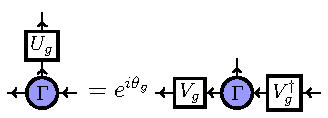
\includegraphics[width=0.6\columnwidth]{group_sym.pdf}.
\end{center}
This equation can be rewritten and solved as an eigenvector problem;
for an MPS with a nondegenerate largest transfer matrix eigenvalue,
this equation is guaranteed have a unique solution where the eigenvalue $e^{i \theta_g}$
is the largest eigenvalue of the eigenvector problem.

The solutions $V_g$ have two important properties: they are only defined up to a phase,
and they are guaranteed to commute with the diagonal matrix $\Lambda$ of Schmidt weights.  

Due to the first property, these operators are not guaranteed to form a linear
representation of the group of on-site symmetries, but in general could make
up a projective representation, satisfying
$$V_g V_h = e^{i \omega(g, h)} V_{gh}.$$ 
It is not always possible to absorb these phases into the definitions of the $V_g$.
The set of equivalent classes of phases $\omega(g, h)$ 
under redefinitions $V_g \to \alpha(g)V_g$ is called $H^2(G, U(1))$, the second group 
cohomology with $U(1)$ coefficients. 

For all the groups discussed in this paper, the group cohomology classes are labeled by
elements of a discrete abelian group - these discrete classes cannot be connected to each other
continuously. Physically, only a phase transition or breaking the symmetry allows one to connect
the different projective symmetry actions. 
Additionally, the classification of projective representations for the on-site symmetry group 
$U(1) \times \mathbb{Z}_W$ representing charge and translation around the cylinder is trivial. 
Thus, these edge symmetries can be taken to act linearly, 
and all Schmidt states can always be simultaneously assigned charge and momentum eigenvalues,
as in Figure~\ref{fig:ESL910}.

The second property guarantees that the $V_g$ only mixes exactly degenerate Schmidt states.
The action of $V_g$ must have the same phases $\omega(g, h)$ on each degenerate block of Schmidt 
states, so the projective representation can be nontrivial on any block only if every Schmidt 
state throughout the entire spectrum is degenerate. The degeneracy will be protected by the 
symmetry if and only if the $V_g$ form a nontrivial projective representation. Therefore
this 1D SPT analysis can only potentially give a nontrival answer for the odd $W$ states 
of the HFBI, where this exact degeneracy is seen throughout the spectrum. Nonetheless, we find 
there are no on-site symmetries of the wavefunction that can be used to explain the degenerate
entanglement spectrum of the odd $W$ HFBI states. Instead we must use an inversion symmetry. 

The MPS analysis of inversion symmetry works similarly. We will consider in general any symmetry  
$h$ of the wavefunction that squares to the identity and that can be written in the MPS as the 
product of an on-site symmetry action $U_h$ and a transpose of the site tensor.
This will include an inversion of the honeycomb lattice - equivalent to a 180 degree rotation 
about the center of any plaquette, which we label $\I = \I_y \I_x$, and the combination of
inversion with on-site symmetries. In addition, by blocking two site-tensors together, we
can write the reflection symmetry $\I_y$ in this form as well. In this scenario, the 
edge symmetry action satisfies
\begin{center}
\beq
\label{eq:onsitesym}
\eeq
\vskip-5em
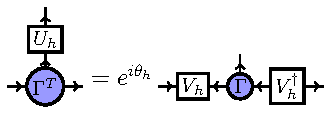
\includegraphics[width=0.6\columnwidth]{inv_sym.pdf}.
\end{center}
The map $V_{h}$ is also computed as a dominant eigenvector. 

For the HFBI, the symmetry group respected by the cylinder geometry is
$U(1) \times (\mathbb{Z}_W \rtimes \mathbb{Z}_2)
\times \mathbb{Z}_2^P \times \mathbb{Z}_2^T$, where the factors refer to charge
symmetry, translation around the cylinder, $\I_x$, $\I_y$, and $\tau$ respectively.
The $P$ and $T$ denote space-reversing and time-reversing symmetries, and signify
that they should be treated as antiunitary when computing the cohomology class
$H^2(U(1) \times (\mathbb{Z}_W \rtimes \mathbb{Z}_2)
\times \mathbb{Z}_2^P \times \mathbb{Z}_2^T ; U(1))$. Many of the non-trivial projective
representations of such a complicated group will remain projective when the symmetry is
restricted to a subgroup - in this case, the full symmetry is not needed to protect the 
entanglement degeneracy. As shown in Table~\ref{table:sym}, the projective representation 
corresponding to the HFBI state can indeed be protected by any one of a number of subgroups 
of the full symmetry group, all involving inversions and charge parity.

The symmetry actions - both on-site and inversion symmetries -
are computed in the Schmidt basis, but can be transformed
into the basis $\vket{\{\sigma_i\}}$ determined by the virtual legs of the PEPS in
Figure~\ref{fig:FBI_PEPS_2}. 
Since
$$
V_{\mathcal{\pi} \mathcal{I}} V_{\mathcal{\pi} \mathcal{I}}^* = -I,
$$

the representation is in the nontrivial class of

$$
H^2(\mathbb{Z}_2^P; U(1)) = \mathbb{Z}_2.
$$


\section{Mode expansion and symmetry action of free-boson CFT}
\label{Appendix:CFT}

\section{Variants on the HFBI wavefunction}
\label{Appendix:Variants}